%!TEX program = xelatex
\documentclass[11pt,twoside,openany,x11names,svgnames]{memoir}



%宏包使用
\usepackage[UTF8,cap,nofonts]{ctex} %,fancyhdr,hyperref winfonts,nofonts

\usepackage{lmodern}
\usepackage{wallpaper}
\usepackage{tikz}
\usetikzlibrary{shapes,positioning}

\usepackage{lipsum}
\usepackage[ISBN=978-80-85955-35-4]{ean13isbn}

%生成书签
\usepackage[CJKbookmarks, colorlinks, bookmarksnumbered=true,pdfstartview=FitH,linkcolor=black]{hyperref} 

%\usepackage[usenames,dvipsnames]{color}   % 支持彩色
\usepackage{color} 
\usepackage{everb} 
\usepackage{keyval, xcolor, calc,ifthen}

\usepackage{booktabs}
\usepackage{float}
\usepackage{indentfirst}
\usepackage[pagestyles]{titlesec}
\usepackage{titletoc}

\usepackage{hypernat}
\usepackage{algpseudocode}
\usepackage{algorithm}
\usepackage{tikz}

\usepackage{listings} %源码宏包
\usepackage{xcolor}   %颜色宏包,语法高亮需要
\usepackage{ulem}



%格式设置
% set up fonts
  \setCJKmainfont[BoldFont={Adobe Heiti Std},ItalicFont={Adobe Kaiti Std}]{Adobe Song Std}
  \setCJKsansfont{Adobe Heiti Std}
  \setCJKmonofont{Adobe Kaiti Std}
  \setCJKfamilyfont{song}{Adobe Song Std}
  \setCJKfamilyfont{hei}{Adobe Heiti Std}
  \setCJKfamilyfont{fs}{Adobe Fangsong Std}
  \setCJKfamilyfont{kai}{Adobe Kaiti Std}
%% Custom stock paper and page size
\setstocksize{303mm}{216mm}
\settrimmedsize{\stockheight}{\stockwidth}{*}

%% Adjust margins around typeblock
\setlrmarginsandblock{23mm}{18mm}{*}
\setulmarginsandblock{23mm}{23mm}{*}

%% Header and footer heights
\setheadfoot{\baselineskip}{10mm}
\setlength\headsep{7mm}

%% To apply and enforce layout
\checkandfixthelayout

%% Command to hold chapter illustration image
\newcommand\chapterillustration{}


%% Define a fancy chapter style
\makechapterstyle{FancyChap}{
%% Vertical Space before main text starts
\setlength\beforechapskip{0pt}
\setlength\midchapskip{0pt}
\setlength\afterchapskip{137mm}
%% Will print chapter number and title
%% in one go ourselves
\renewcommand*\printchaptername{}
\renewcommand*\printchapternum{}
%%% Re-define how the chapter title is printed
\def\printchaptertitle##1{

%=========定义颜色===================================
%\definecolor{blueblack}{cmyk}{0,0,0,0.35}%浅黑
\definecolor{lightgray}{gray}{0.9}
\definecolor{blueblack}{RGB}{0,0,135}
\definecolor{darkblue}{cmyk}{1,0,0,0}%纯蓝
\definecolor{lightblue}{cmyk}{0.15,0,0,0}%浅蓝
%====================================================



%% Background image at top of page
\ThisULCornerWallPaper{1}{\chapterillustration}
%% Draw a semi-transparent rectangle across the top
\tikz[overlay,remember picture]
  \fill[fill=LightSalmon1,opacity=.7]
  (current page.north west) rectangle 
  ([yshift=-3cm] current page.north east);
  %% Check if on an odd or even page
  \strictpagecheck\checkoddpage
  %% On odd pages, "logo" image at lower right
  %% corner; Chapter number printed near spine
  %% edge (near the left); chapter title printed
  %% near outer edge (near the right).
  \ifoddpage{
    \ThisLRCornerWallPaper{.35}{fern_mo_01}
    \begin{tikzpicture}[overlay,remember picture]
    \node[anchor=south west,
      xshift=20mm,yshift=-30mm,
      font=\sffamily\bfseries\huge] 
      at (current page.north west) 
      {\chaptername\chapternamenum\thechapter};
    \node[fill=Sienna!80!black,text=white,
      font=\Huge\bfseries, 
      inner ysep=12pt, inner xsep=20pt,
      rounded rectangle,anchor=east, 
      xshift=-20mm,yshift=-30mm] 
      at (current page.north east) {##1};
    \end{tikzpicture}
  }
  %% On even pages, "logo" image at lower left
  %% corner; Chapter number printed near outer
  %% edge (near the right); chapter title printed
  %% near spine edge (near the left).
  \else {
    \ThisLLCornerWallPaper{.35}{fern_mo_01}
    \begin{tikzpicture}[overlay,remember picture]
    \node[anchor=south east,
      xshift=-20mm,yshift=-30mm,
      font=\sffamily\bfseries\huge] 
      at (current page.north east)
      {\chaptername\chapternamenum\thechapter};
    \node[fill=Sienna!80!black,text=white,
      font=\Huge\bfseries,
      inner sep=12pt, inner xsep=20pt,
      rounded rectangle,anchor=west,
      xshift=20mm,yshift=-30mm] 
      at ( current page.north west) {##1};
    \end{tikzpicture}
  }
  \fi
}
}


%% Define a fancy chapter style for unnumbered
%% chapters (e.g. the Table of Contents)
\makechapterstyle{FancyUnnumberedChap}{
%% Vertical Space before main text starts
\setlength\beforechapskip{0pt}
\setlength\midchapskip{0pt}
\setlength\afterchapskip{47mm}
%% Will print chapter number and title
%% in one go ourselves
\renewcommand*\printchaptername{}
\renewcommand*\printchapternum{}
%%% Re-define how the chapter title is printed
\def\printchaptertitle##1{
%% Draw a semi-transparent rectangle across the top
\tikz[overlay,remember picture]
  \fill[fill=LightSalmon1,opacity=.7]
  (current page.north west) rectangle 
  ([yshift=-3cm] current page.north east);
  %% Check if on an odd or even page
  \strictpagecheck\checkoddpage
  \ifoddpage{
    \begin{tikzpicture}[remember picture, overlay]
    \node[fill=Sienna!80!black,text=white,
      font=\Huge\bfseries, 
      inner ysep=12pt, inner xsep=20pt,
      rounded rectangle,anchor=east, 
      xshift=-20mm,yshift=-30mm] 
      at (current page.north east) {##1};
    \end{tikzpicture}
  }
  \else {
    \begin{tikzpicture}[remember picture, overlay]
    \node[fill=Sienna!80!black,text=white,
      font=\Huge\bfseries,
      inner sep=12pt, inner xsep=20pt,
      rounded rectangle,anchor=west,
      xshift=20mm,yshift=-30mm] 
      at ( current page.north west) {##1};
    \end{tikzpicture}
  }
  \fi
}
}


%% Set the uniform width of the colour box
%% displaying the page number in footer
%% to the width of "99"
\newlength\pagenumwidth
\settowidth{\pagenumwidth}{99}

%% Define style of page number colour box
\tikzset{pagefooter/.style={
anchor=base,font=\sffamily\bfseries\small,
text=white,fill=Sienna!80!black,text centered,
text depth=17mm,text width=\pagenumwidth}}

%% Concoct some colours of our own
\definecolor[named]{GreenTea}{HTML}{CAE8A2}
\definecolor[named]{MilkTea}{HTML}{C5A16F}

%% Sometimes I prefer not to upper-case my
%% running headers
\nouppercaseheads

%%%%%%%%%%
%%% Re-define running headers on non-chapter odd pages
%%%%%%%%%%
\makeoddhead{headings}
%% Left header is empty but I'm using it as a hook to paint the
%% background rectangles underneath everything else
{\begin{tikzpicture}[remember picture,overlay]
\fill[MilkTea!25!white] (current page.north east) 
	rectangle (current page.south west);
\fill[white, rounded corners] 
	([xshift=-10mm,yshift=-20mm]current page.north east) rectangle 	
	([xshift=15mm,yshift=17mm]current page.south west);
\end{tikzpicture}}%
%% Blank centre header
{}%
%% Display a decorate line and the right mark (chapter title)
%% at right end
{\begin{tikzpicture}[xshift=-.75\baselineskip,yshift=.25\baselineskip,remember picture, overlay,fill=GreenTea,draw=GreenTea]\fill circle(3pt);\draw[semithick](0,0) -- (current page.west |- 0,0);\end{tikzpicture}\sffamily\itshape\small\rightmark}

%%%%%%%%%%
%%% Re-define running footers on odd pages
%%% i.e. display the page number on the right
%%%%%%%%%%
\makeoddfoot{headings}{}{}{%
\tikz[baseline]\node[pagefooter]{\thepage};}
\makeoddfoot{plain}{}{}{\tikz[baseline]\node[pagefooter]{\thepage};}

%%%%%%%%%%
%%% Re-define running headers on non-chapter even pages
%%%%%%%%%%
\makeevenhead{headings}
%% Draw the background rectangles; then the left mark (section
%% title) and the decorate line
{{\begin{tikzpicture}[remember picture,overlay]
\fill[MilkTea!25!white] (current page.north east) rectangle (current page.south west);
\fill[white, rounded corners] ([xshift=-15mm,yshift=-20mm]current page.north east) rectangle ([xshift=10mm,yshift=17mm]current page.south west);
\end{tikzpicture}}%
\sffamily\itshape\small\leftmark\ 
\begin{tikzpicture}[xshift=.5\baselineskip,yshift=.25\baselineskip,remember picture, overlay,fill=GreenTea,draw=GreenTea]\fill (0,0) circle (3pt); \draw[semithick](0,0) -- (current page.east |- 0,0 );\end{tikzpicture}}{}{}
\makeevenfoot{headings}{\tikz[baseline]\node[pagefooter]{\thepage};}{}{}
\makeevenfoot{plain}{\tikz[baseline]\node[pagefooter]{\thepage};}
%% Empty centre and right headers on even pages
{}{}

\setlength\parindent{0pt}
\begin{document}


%封面设置
\frontmatter

%%%%%%%%%%%%%%
%% 封面页
%%%%%%%%%%%%%%

%% No header nor footer on the cover
\thispagestyle{empty}

%% Cover illustration
\ThisLLCornerWallPaper{1}{grapes-in-my-studio-little-too-much-dust}

%% Bar across the top
\tikz[remember picture,overlay]%
\node[fill=Sienna,text=white,font=\LARGE\bfseries,text=Cornsilk,%
minimum width=\paperwidth,minimum height=5em,anchor=north]%
at (current page.north){Exercises in \LaTeX};

\vspace*{2\baselineskip}

{\bfseries\itshape\color{LightGoldenrod!50!Gold}\fontsize{36pt}{46pt}\selectfont
The Linux Command  \par 
Line(中文版) \par}

\vspace*{2\baselineskip}

{\LARGE\color{LightGoldenrod}
一本绝对值得一读的 \scshape{好书}\par
}

\tikz[remember picture,overlay]%
\node[fill=Sienna,font=\LARGE\bfseries,text=Cornsilk,%
minimum width=\paperwidth,minimum height=3em,anchor=south]%
 at (current page.south) {翻译:好奇猫团队 ~~PDF制作:UnkelTao};


\begin{center}
\LARGE\bfseries\color{SaddleBrown!30!black}

\end{center}

\cleartorecto


%%%%%%
%结束封面
%%%%%%

%罗马计数
\frontmatter


%章节Style设置
%% Invoke fancy unnumbered chapter style
%% for the table of contents
\chapterstyle{FancyUnnumberedChap}

\tableofcontents*
%% Main matter starts here; resets page-numberings to arabic numeral 1

%% Invoke the FancyChap chapter style
\chapterstyle{FancyChap}

\lstset{
	    %numbers=left, %设置行号位置
        %numberstyle=\tiny, %设置行号大小
        keywordstyle=\color{blue}, %设置关键字颜色
        commentstyle=\color[cmyk]{1,0,1,0}, %设置注释颜色
        frame=single, %设置边框格式
        escapeinside=``, %逃逸字符(1左面的键),用于显示中文
        breaklines, %自动折行
        extendedchars=false, %解决代码跨页时,章节标题,页眉等汉字不显示的问题
        xleftmargin=2em,xrightmargin=2em, aboveskip=1em, %设置边距
        tabsize=4, %设置tab空格数
        showspaces=false %不显示空格
       } %源代码风格

\XeTeXlinebreaklocale "zh"

% \renewcommand{\chaptername}{第\CJKnumber{\thechapter}章}
% \newcommand{\sectionname}{节}
\renewcommand{\figurename}{图}
\renewcommand{\tablename}{表}
% \renewcommand{\bibname}{参考文献}
% \renewcommand{\contentsname}{目~录}
% \renewcommand{\listfigurename}{图~目~录}
% \renewcommand{\listtablename}{表~目~录}
% \renewcommand{\indexname}{索~引}
% \renewcommand{\abstractname}{\Large{摘~要}}
% \newcommand{\keywords}[1]{\\ \\ \textbf{关~键~词}:#1}
% \titleformat{\chapter}[block]{\center\Large\bf}{\chaptername}{20pt}{}
% \titleformat{\section}[block]{\large\bf}{\thesection}{10pt}{}



% 引言
%% Public domain image from
%% http://www.public-domain-image.com/objects/computer-chips/slides/six-computers-chips-circuits.html
\renewcommand\chapterillustration{cherry-tomatos.jpg}
\chapter{引言}
\label{引言}


我想给大家讲个故事。

\par 故事内容不是 Linus Torvalds 在1991年怎样写了 Linux 内核的第一个版本, 因为这些内容你可以在许多 Linux 书籍中读到。我也不想告诉你,更早之前,Richard Stallman 是如何开始 GNU 项目,设计了一个免费的类似 Unix 的操作系统。那也是一个很有意义的故事, 但大多数 Linux 书籍也讲到了它。

\par 我想告诉大家一个你如何才能夺回计算机管理权的故事。

\par 在20世纪70年代末,我刚开始和计算机打交道时,正进行着一场革命,那时的我还是一名大学生。 微处理器的发明,让你我这样的普通老百姓也有可能真正拥有一台计算机。今天, 人们很难想象,只有大企业和强大的政府才能够拥有计算机的世界,是怎样的一个世界。 让我说,你想不出多少来。

\par 今天,世界已经截然不同了。计算机遍布各个领域,从小手表到大型数据中心,及大小介于它们之间的每件东西。 除了随处可见的计算机之外,我们还有一个无处不在的连接所有计算机的网络。这已经开创了一个人们可以 自我营造和自由创作的奇妙的新时代,但在过去的二三十年里,一些事情仍然在发生着改变。一个大公司不断地把它的 管理权强加到世界上绝大多数的计算机上,并且决定你对计算机的操作权力。幸运地是,来自世界各地的人们, 正积极努力地做些事情来改变这种境况。通过编写自己的软件,他们一直在为维护电脑的管理权而战斗着。 他们建设着 Linux。

\par 一提到 Linux,许多人都会说到“自由”,但我不认为他们都知道“自由”的真正涵义。“自由”是一种权力, 它决定你的计算机能做什么,同时,只有知道计算机正在做什么你才能够拥有这种“自由”。 “自由”是指一台没有任何秘密的计算机,你可以从它那里了解一切,只要你用心的去寻找。

\section{ls 乐趣}

有充分的理由证明,ls 可能是用户最常使用的命令。通过它,我们可以知道目录的内容,以及各种各样重要文件和目录的 属性。正如我们所知道的,只简单的输入 ls 就能看到在当前目录下所包含的文件和子目录列表。

\begin{lstlisting}
[me@linuxbox ~]$ ls
Desktop Documents Music Pictures Publica Templates Videos 
\end{lstlisting}

\par 除了当前工作目录以外,也可以列出指定目录的内容,就像这样:

\begin{lstlisting}
me@linuxbox ~]$ ls /usr
bin games   kerberos    libexec  sbin   src
etc include lib         local    share  tmp 
\end{lstlisting}

\par 甚至可以列出多个指定目录的内容。在这个例子中,将会列出用户主目录(用字符“~”代表)和/usr 目录的内容:

\begin{lstlisting}
[me@linuxbox ~]$ ls ~ /usr
/home/me:
Desktop  Documents  Music  Pictures  Public  Templates  Videos

/usr:
bin  games      kerberos  libexec  sbin   src
etc  include    lib       local    share  tmp 
\end{lstlisting}

\par 我们也可以改变输出格式,来得到更多的细节:

\begin{lstlisting}
[me@linuxbox ~]$ ls -l
total 56
drwxrwxr-x 2  me  me  4096  2007-10-26  17:20  Desktop
drwxrwxr-x 2  me  me  4096  2007-10-26  17:20  Documents
drwxrwxr-x 2  me  me  4096  2007-10-26  17:20  Music
drwxrwxr-x 2  me  me  4096  2007-10-26  17:20  Pictures
drwxrwxr-x 2  me  me  4096  2007-10-26  17:20  Public
drwxrwxr-x 2  me  me  4096  2007-10-26  17:20  Templates
drwxrwxr-x 2  me  me  4096  2007-10-26  17:20  Videos
\end{lstlisting}

\par 使用 ls 命令的“-l”选项,则结果以长模式输出。


\subsection{选项和参数}
我们将学习一个非常重要的知识点,大多数命令是如何工作的。命令名经常会带有一个或多个用来更正命令行为的选项, 更进一步,选项后面会带有一个或多个参数,这些参数是命令作用的对象。所以大多数命令看起来像这样:

\begin{lstlisting}
command -options arguments
\end{lstlisting}

\par 大多数命令使用的选项,是由一个中划线加上一个字符组成,例如,“-l”,但是许多命令,包括来自于 GNU 项目的命令,也支持长选项,长选项由两个中划线加上一个字组成。当然, 许多命令也允许把多个短选项串在一起使用。下面这个例子,ls 命令有两个选项, “l” 选项产生长格式输出,“t”选项按文件修改时间的先后来排序。

\begin{lstlisting}
[me@linuxbox ~]$ ls -lt
\end{lstlisting}

\par 加上长选项 “–reverse”,则结果会以相反的顺序输出:

\begin{lstlisting}
[me@linuxbox ~]$ ls -lt --reverse
\end{lstlisting}

\par ls 命令有大量的选项。表3-1列出了最常使用的选项。

\begin{table}[ht!]
% increase table row spacing, adjust to taste
%\renewcommand{\arraystretch}{1.2}
\caption{ls 命令选项}
\label{table_example}
\centering
\begin{tabular}{p{1.5cm}p{3.5cm}p{10cm}}
%\begin{tabular}{c|c|c}
\hline
%\begin{tabular}{|p{0.18\textwidth}|p{0.36\textwidth}|p{0.36\textwidth}|}
 选项 & 长选项 & 描述 \\
\hline
 -a & --all & 列出所有文件,甚至包括文件名以圆点开头的隐藏文件。 \\
-d & --directory & 通常,如果指定了目录名,ls 命令会列出这个目录中的内容,而不是目录本身。 把这个选项与-l 选项结合使用,可以看到所指定目录的详细信息,而不是目录中的内容。\\
-F & --classify	& 这个选项会在每个所列出的名字后面加上一个指示符。例如,如果名字是 目录名,则会加上一个``/''字符。 \\
-h & --human-readable & 以长格式列出。以人们可读的格式,而不是以字节数来显示文件的大小。\\
-l & & 以长格式显示结果。\\
-r & --reverse & 以相反的顺序来显示结果。通常,ls 命令的输出结果按照字母升序排列。 \\
-S & & 命令输出结果按照文件大小来排序。\\
-t & & 按照修改时间来排序。\\
\hline
\end{tabular}
\end{table}


\subsection{深入研究长格式输出}
正如我们先前知道的,“-l”选项导致 ls 的输出结果以长格式输出。这种格式包含大量的有用信息。下面的例子目录来自 于 Ubuntu 系统:
(注:由于排版原因,删除了原文的的一部分.)
\begin{lstlisting}
-rw-r--r-- 1 root root 3576296 2007-04-03 11:05 Experience ubuntu.ogg
-rw-r--r-- 1 root root 1186219 2007-04-03 11:05 kubuntu-leaflet.png 
-rw-r--r-- 1 root root   47584 2007-04-03 11:05 logo-Edubuntu.png 
-rw-r--r-- 1 root root   44355 2007-04-03 11:05 logo-Kubuntu.png
-rw-r--r-- 1 root root   34391 2007-04-03 11:05 logo-Ubuntu.png
-rw-r--r-- 1 root root   32059 2007-04-03 11:05 oo-cd-cover.odf
\end{lstlisting}

\par 选一个文件,来看一下各个输出字段的含义(表3-2):

\begin{table}[ht!]
% increase table row spacing, adjust to taste
%\renewcommand{\arraystretch}{1.2}
\caption{ls 长格式列表的字段}
\label{table_example}
\centering
\begin{tabular}{p{4cm}p{11cm}}
%\begin{tabular}{c|c|c}
\hline
%\begin{tabular}{|p{0.18\textwidth}|p{0.36\textwidth}|p{0.36\textwidth}|}
 字段 & 含义 \\
 \hline 
 -rw-r--r--	& 对于文件的访问权限。第一个字符指明文件类型。在不同类型之间,开头的“-”说明是一个普通文件,“d”表明是一个目录。其后三个字符是文件所有者的访问权限,再其后的三个字符是文件所属组中成员的访问权限,最后三个字符是其他所 有人的访问权限。这个字段的完整含义将在第十章讨论。\\
1 & 文件的硬链接数目。参考随后讨论的关于链接的内容。 \\
root & 文件属主的用户名。 \\
root & 文件所属用户组的名字。 \\
32059 & 以字节数表示的文件大小。\\
2007-04-03 11:05 & 上次修改文件的时间和日期。 \\
oo-cd-cover.odf	& 文件名。 \\
\hline

\end{tabular}
\end{table}

\section{mkdir - 创建文件夹} % (fold)
\label{sec:mkdir_创建文件夹}
mkdir 命令是用来创建目录的。它这样工作:
\begin{lstlisting}
mkdir directory...
\end{lstlisting}
\par \textbf{注意表示法}: 在描述一个命令时(如上所示),当有三个圆点跟在一个命令的参数后面, 这意味着那个参数可以重复,就像这样:
\begin{lstlisting}
mkdir dir1
\end{lstlisting}
\par 会创建一个名为”dir1”的目录,而
\begin{lstlisting}
mkdir dir1 dir2 dir3
\end{lstlisting}
\par 会创建三个目录,名为``dir1'', ``dir2'', ``dir3''。


% section mkdir_创建文件夹 (end)

\section{用 less 浏览文件内容} % (fold)
\label{sec:用_less_浏览文件内容}

less 命令是一个用来浏览文本文件的程序。纵观 Linux 系统,有许多人类可读的文本文件。less 程序为我们检查文本文件 提供了方便。

\fboxrule=6pt \fboxsep=4pt
\begin{colorboxed}[boxcolor=lightgray,bgcolor=white]
\subsection{什么是``文本''}
在计算机中,有许多方法可以表达信息。所有的方法都涉及到,在信息与一些数字之间确立一种关系,而这些数字可以 用来表达信息。毕竟,计算机只能理解数字,这样所有的数据都被转换成数值表示法。

\par 有些数值表达法非常复杂(例如压缩的视频文件),而其它的就相当简单。最早也是最简单的一种表达法,叫做 ASCII 文本。ASCII(发音是"As-Key")是美国信息交换标准码的简称。这是一个简单的编码方法,它首先 被用在电传打字机上,用来实现键盘字符到数字的映射。

\par 文本是简单的字符与数字之间的一对一映射。它非常紧凑。五十个字符的文本翻译成五十个字节的数据。文本只是包含 简单的字符到数字的映射,理解这点很重要。它和一些文字处理器文档不一样,比如说由微软和 OpenOffice.org 文档 编辑器创建的文件。这些文件,和简单的 ASCII 文件形成鲜明对比,它们包含许多非文本元素,来描述它的结构和格式。 普通的 ASCII 文件,只包含字符本身,和一些基本的控制符,像制表符,回车符及换行符。纵观 Linux 系统,许多文件 以文本格式存储,也有许多 Linux 工具来处理文本文件。甚至 Windows 也承认这种文件格式的重要性。著名的 NOTEPAD.EXE 程序就是一个 ASCII 文本文件编辑器。
\end{colorboxed}

\par 为什么我们要查看文本文件呢? 因为许多包含系统设置的文件(叫做配置文件),是以文本格式存储的,阅读它们 可以更深入的了解系统是如何工作的。另外,许多系统所用到的实际程序(叫做脚本)也是以这种格式存储的。 在随后的章节里,我们将要学习怎样编辑文本文件,为的是修改系统设置,还要学习编写自己的脚本文件,但现在我们只是看看它们的内容而已。

\par less 命令是这样使用的:

\begin{lstlisting}
less filename
\end{lstlisting}

\par 一旦运行起来,less 程序允许你前后滚动文件。例如,要查看一个定义了系统中全部用户身份的文件,输入以下命令:
\begin{lstlisting}
[me@linuxbox ~]$ less /etc/passwd
\end{lstlisting}

\par 一旦 less 程序运行起来,我们就能浏览文件内容了。如果文件内容多于一页,那么我们可以上下滚动文件。按下“q”键, 退出 less 程序。

\par 下表列出了 less 程序最常使用的键盘命令。
\begin{table}[ht!]
% increase table row spacing, adjust to taste
%\renewcommand{\arraystretch}{1.2}
\caption{less 命令}
\label{table3}
\centering
\begin{tabular}{p{4cm}p{11cm}}
%\begin{tabular}{c|c|c}
\hline
%\begin{tabular}{|p{0.18\textwidth}|p{0.36\textwidth}|p{0.36\textwidth}|}
命令 & 行为\\

\hline
Page UP or b &	向后翻滚一页\\
Page Down or space & 向前翻动一页 \\
UP Arrow & 向前移动一行\\
Down Arrow &	向后移动一行\\
G	& 移动到最后一行\\
1G or g	& 移动到开头一行\\
/charaters	& 向前查找指定的字符串\\
n	& 向前查找下一个出现的字符串,这个字符串是之前所指定查找的\\
h	& 显示帮助屏幕\\
q	& 退出 less 程序\\
\hline
\end{tabular}
\end{table}

\fboxrule=6pt \fboxsep=4pt
\begin{colorboxed}[boxcolor=lightgray,bgcolor=white]
\subsection{less 就是 more(禅语:色即是空)}

ess 程序是早期 Unix 程序 more 的改进版。“less” 这个名字,对习语 “less is more” 开了个玩笑, 这个习语是现代主义建筑师和设计者的座右铭。

\par less 属于”页面调度器”程序类,这些程序允许通过页方式,在一页中轻松地浏览长长的文本文档。然而 more 程序只能向前分页浏览,而 less 程序允许前后分页浏览,它还有很多其它的特性。
\end{colorboxed}


% section 用_less_浏览文件内容 (end)

\section{更改当前工作目录} % (fold)
\label{sec:更改当前工作目录}
\par 要更改工作目录(此刻,我们站在树形迷宫里面),我们用 cd 命令。输入 cd, 然后输入你想要的工作目录的路径名,就能实现愿望。路径名就是沿着目录树的分支 到达想要的目录,期间所经过的路线。路径名可通过两种方式来指定,一个是绝对路径, 另一个是相对路径。首先处理绝对路径。

\subsection{绝对路径} % (fold)
\label{ssub:绝对路径}
绝对路径开始于根目录,紧跟着目录树的一个个分支,一直到达期望的目录或文件。 例如,你的系统中有一个目录,大多数系统程序都安装在这个目录下。这个目录的 路径名是 /usr/bin。它意味着从根目录(用开头的“/”表示)开始,有一个叫 “usr” 的 目录包含了目录 “bin”。
\begin{lstlisting}
[me@linuxbox ~]$ cd /usr/bin
[me@linuxbox bin]$ pwd
/usr/bin
[me@linuxbox bin]$ ls
...Listing of many, many files ...
\end{lstlisting}
\par 我们把工作目录转到 /usr/bin 目录下,里面装满了文件。注意 shell 提示符是怎样改变的。 为了方便,通常设置提示符自动显示工作目录名。
% subsection 绝对路径 (end)

\subsection{相对路径} % (fold)
\label{sub:相对路径}
绝对路径从根目录开始,直到它的目的地,而相对路径开始于工作目录。 一对特殊符号来表示相对位置,在文件系统树中。这对特殊符号是 ``.'' (点) 和 ``..'' (点点)。

\par 符号 ``.'' 指的是工作目录,``..'' 指的是工作目录的父目录。下面的例子说明怎样使用它。 再次更改工作目录到 /usr/bin:
\begin{lstlisting}
[me@linuxbox ~]$ cd /usr/bin
[me@linuxbox bin]$ pwd
/usr/bin
\end{lstlisting}

\par 好的,比方说更改工作目录到 /usr/bin 的父目录 /usr。可以通过两种方法来实现。或者使用绝对路径名:

\begin{lstlisting}
[me@linuxbox bin]$ cd /usr
[me@linuxbox usr]$ pwd
/usr
\end{lstlisting}

\par 或者, 使用相对路径:

\begin{lstlisting}
[me@linuxbox bin]$ cd ..
[me@linuxbox usr]$ pwd
/usr
\end{lstlisting}

\par 两种不同的方法,一样的结果。我们应该选哪一个呢? 输入量最少的那个。

\par 同样地,从目录/usr/到/usr/bin 也有两种途径。或者使用绝对路径:

\begin{lstlisting}
[me@linuxbox usr]$ cd /usr/bin
[me@linuxbox bin]$ pwd
/usr/bin
\end{lstlisting}

\par 或者,用相对路径:

\begin{lstlisting}
[me@linuxbox usr]$ cd ./bin
[me@linuxbox bin]$ pwd
/usr/bin
\end{lstlisting}

\par 有一件很重要的事,我必须指出来。在几乎所有的情况下,你可以省略”./”。它是隐含地。输入:
\begin{lstlisting}
[me@linuxbox usr]$ cd bin
\end{lstlisting}

\par 实现相同的效果,如果不指定一个文件的目录,那它的工作目录会被假定为当前工作目录。

% subsection 相对路径 (end)

\subsubsection{有用的快捷键} % (fold)
\label{ssub:有用的快捷键}
在表2-1中,列举出了一些快速改变当前工作目录的有效方法。


\begin{table}[ht!]
% increase table row spacing, adjust to taste
%\renewcommand{\arraystretch}{1.2}
\caption{cd 快捷键}
\label{table_example}
\centering
\begin{tabular}{c|c}
\hline
%\begin{tabular}{|p{0.18\textwidth}|p{0.36\textwidth}|p{0.36\textwidth}|}
 快捷键 & 运行结果 \\
\hline
  cd	& 更改工作目录到主目录。 \\
  cd -	& 更改工作目录到先前的工作目录。\\
cd ~user\_name	& 更改工作目录到用户主目录。例如, cd ~bob 会更改工作目录到用户“bob”的主目录。\\
\hline
\end{tabular}
\end{table}

% subsubsection 有用的快捷键 (end)
\fboxrule=6pt \fboxsep=4pt
\begin{colorboxed}[boxcolor=lightgray,bgcolor=white]
\subsubsection{关于文件名的重要规则}
\begin{enumerate}
	\item 以 ``.'' 字符开头的文件名是隐藏文件。这仅表示,ls 命令不能列出它们, 除非使用 ls -a 命令。当你创建帐号后,几个配置帐号的隐藏文件被放置在 你的主目录下。稍后,我们会仔细研究一些隐藏文件,来定制你的系统环境。 另外,一些应用程序也会把它们的配置文件以隐藏文件的形式放在你的主目录下面。
	\item 文件名和命令名是大小写敏感的。文件名 “File1” 和 “file1” 是指两个不同的文件名。
	\item Linux 没有“文件扩展名”的概念,不像其它一些系统。可以用你喜欢的任何名字 来给文件起名。文件内容或用途由其它方法来决定。虽然类似 Unix 的操作系统, 不用文件扩展名来决定文件的内容或用途,但是应用程序会。
	\item 虽然 Linux 支持长文件名,文件名可能包含空格,标点符号,但标点符号仅限 使用 ``.'',``-'',下划线。最重要的是,不要在文件名中使用空格。如果你想表示词与 词间的空格,用下划线字符来代替。过些时候,你会感激自己这样做。
\end{enumerate}
\end{colorboxed}
% section 更改当前工作目录 (end)

\section{怎样阅读这本书} % (fold)
\label{sec:怎样阅读这本书}

从头到尾的阅读。它并不是一本技术参考手册,实际上它更像一本故事书,有开头,过程,结尾。

\subsection{前提条件} % (fold)
\label{ssub:_前提条件}
为了使用这本书,你需要安装 Linux 操作系统。你可以通过两种方式,来完成安装。
\begin{itemize}
\item 1. 在一台(不是很新)的电脑上安装 Linux。你选择哪个 Linux 发行版安装,是无关紧要的事。 虽然大多数人一开始选择安装 Ubuntu, Fedora, 或者 OpenSUSE。如果你拿不定主意,那就先试试 Ubuntu。 由于主机硬件配置不同,安装 Linux 时,你可能不费吹灰之力就装上了,也可能费了九牛二虎之力还装不上。 所以我建议,一台使用了几年的台式机,至少要有256M 的内存,6G 的硬盘可用空间。尽可能避免使用 笔记本电脑和无线网络,在 Linux 环境下,它们经常不能工作。

\item 2. 使用“Live CD.” 许多 Linux 发行版都自带一个比较酷的功能,你可以直接从系统安装盘 CDROM 中运行 Linux, 而不必安装 Linux。开机进入 BIOS 设置界面,更改引导项,设置为“从 CDROM 启动”。
\end{itemize}

\par 不管你怎样安装 Linux,为了练习书中介绍的知识,你需要有超级用户(管理员)权限。

\par 当你在自己的电脑上安装了 Linux 系统之后,就开始一边阅读本书,一边练习吧。本书大部分内容 都可以自己动手练习,坐下来,敲入命令,体验一下吧。



%\lemmabox{

\fboxrule=6pt \fboxsep=4pt
\begin{colorboxed}[boxcolor=lightgray,bgcolor=white]
 \subsubsection{为什么我不叫它“GNU/Linux”}

\par 在某些领域,把 Linux 操作系统称为“GNU/Linux 操作系统.”是比较明智的做法。但“Linux”的问题在于, 没有一个完全正确的方式能为它命名,因为它是由许许多多,分布在世界各地的贡献者们,合作开发而成的。 从技术层面讲,Linux 只是操作系统的内核名字,没别的含义。当然内核非常重要,有了内核, 操作系统才能运行起来,但它并不能构成一个完整的操作系统。

\par Richard Stallman 是一个天才的哲学家,自由软件运动创始人,自由软件基金会创办者,他创建了 GNU 工程, 编写了第一版 GNU C 编译器(gcc),创立了 GNU 通用公共协议(the GPL)等等。 他坚持把 Linux 称为“GNU/Linux”,为的是准确地反映 GNU 工程对 Linux 操作系统的贡献。 然而,GNU 项目早于 Linux 内核,而 GNU 项目的贡献得到了极高的赞誉,再把 GNU 用在 Linux 名字里, 这对其他每个为 Linux 的发展做出重大贡献的程序员来说,就不公平了。

\par 在目前流行的用法中,“Linux”指的是内核以及在一个典型的 Linux 发行版中所包含的所有免费及开源软件; 也就是说,整个 Linux 生态系统,不只有 GNU 项目软件。在操作系统商界,好像喜欢使用单个词的名字, 比如说 DOS, Windows, MacOS, Solaris, Irix, AIX. 所以我选择用流行的命名规则。然而, 如果你喜欢用“GNU/Linux”,当你读这本书时,可以搜索并代替“Linux”。我不介意。
\end{colorboxed}


% subsection _前提条件 (end)
% section 怎样阅读这本书 (end)

\section{拓展阅读} % (fold)
\label{sec:拓展阅读}

\begin{itemize}
	\item Wikipedia 网站上有些介绍本章提到的名人的文章,以下是链接地址:\\
	\url{http://en.wikipedia.org/wiki/Linux_Torvalds}\\
	\url{http://en.wikipedia.org/wiki/Richard_Stallman}
	\item 介绍自由软件基金会及 GNU 项目的网站和文章:\\
	\url{http://en.wikipedia.org/wiki/Free_Software_Foundation}\\
	\url{http://www.fsf.org}\\
	\url{http://www.gnu.org}
	\item Richard Stallman 用了大量的文字来叙述“GNU/Linux”的命名问题,可以浏览以下网页:\\
	\url{http://www.gnu.org/gnu/why-gnu-linux.html}\\
	\url{http://www.gnu.org/gnu/why-gnu-linux.html}\\
	\url{http://www.gnu.org/gnu/gnu-linux-faq.html#tools}
\end{itemize}
% section 拓展阅读 (end)


%阿拉伯计数
\mainmatter

%第一部分
\part{学习Shell}

%第一章
%% Public domain image from
%% http://www.public-domain-image.com/still-life/slides/cherry-tomatos.html
\renewcommand\chapterillustration{cherry-tomatos}
\chapter{什么是 shell}

一说到命令行,我们真正指的是 shell。shell 就是一个程序,它接受从键盘输入的命令, 然后把命令传递给操作系统去执行。几乎所有的 Linux 发行版都提供一个名为 bash 的程序, bash 是 shell 的一种,来自于 GNU 项目。“bash”是“Bourne Again SHell”的首字母缩写, 所指的是这样一个事实,bash 是 sh 的增强版,sh 是最初 Unix 的 shell 程序,由 Steve Bourne 写成。

\section{终端仿真器} % (fold)
\label{sec:终端仿真器}

当使用图形用户界面时,我们需要另一个叫做终端仿真器的程序,去和 shell 交互。 浏览一下我们的桌面菜单,我们可能会找到一个。虽然在菜单里它可能都 被简单地称为“terminal”,但是 KDE 用的是 konsole 程序, 而 GNOME 则使用 gnome-terminal。 还有其他一些终端仿真器可供 Linux 使用,但基本上,它们都是为了完成同样的事情, 让我们能访问 shell。也许,你会喜欢上这个或那个终端,由于它所附加的一系列花俏功能。


% section 终端仿真器 (end)

\section{第一次按键} % (fold)
\label{sec:第一次按键}

好,开始吧。启动终端仿真器!一旦它运行起来,我们应该能够看到一行类似下面文字的输出:\\
\\
\begin{lstlisting}
[me@linuxbox ~]$
\end{lstlisting}

\par 这叫做 shell 提示符,当 shell 准备好了去接受输入时,它就会出现。然而, 它可能会以各种各样的面孔显示,这则取决于不同的 Linux 发行版, 它通常包括你的用户名\@主机名,紧接着当前工作目录(关于它的知识有点多)和一个美元符号。

\par 如果提示符的最后一个字符是``\verb"#"'', 而不是``\textdollar'', 那么这个终端会话就有超级用户权限。 这意味着,我们或者是以根用户的身份登录,或者是我们选择的终端仿真器提供超级用户(管理员)权限。

\par 假定到目前为止,所有事情都进行顺利,那我们试着打字吧。在提示符下敲入 一些乱七八糟的无用数据,如下所示:
\begin{lstlisting}
[me@linuxbox ~]$ kaekfjaeifj
\end{lstlisting}

\par 因为这个命令没有任何意义,所以 shell 会提示错误信息,并让我们再试一下:
\begin{lstlisting}
bash: kaekfjaeifj: command not found
[me@linuxbox ~]$
\end{lstlisting}

\subsection{命令历史}
如果按下上箭头按键,我们会看到刚才输入的命令“kaekfjaeifj”重新出现在提示符之后。 这就叫做命令历史。许多 Linux 发行版默认保存最后输入的500个命令。 按下下箭头按键,先前输入的命令就消失了。

\subsection{移动光标}
可借助上箭头按键,来回想起上次输入的命令。现在试着使用左右箭头按键。 看一下怎样把光标定位到命令行的任意位置?通过使用箭头按键,使编辑命令变得轻松些。

\fboxrule=6pt \fboxsep=4pt
\begin{colorboxed}[boxcolor=lightgray,bgcolor=white]
\subsubsection{关于鼠标和光标}
虽然,shell 是和键盘打交道的,但你也可以在终端仿真器里使用鼠标。X 窗口系统 (使 GUI 工作的底层引擎)内建了一种机制,支持快速拷贝和粘贴技巧。 如果你想高亮一些文本,可以按下鼠标左键,沿着文本拖动鼠标(或者双击一个单词), 那么这些高亮的文本就被拷贝到了一个由 X 管理的缓冲区里面。然后按下鼠标中键, 这些文本就被粘贴到光标所在的位置。试试看。

\par 注意: 不要受诱惑在一个终端窗口里,使用 Ctrl-c 和 Ctrl-v 快捷键,来执行拷贝和粘贴操作。 它们不起作用。对于 shell 来说,这些控制代码有着不同的含义,它们被赋值,早于 Microsoft Windows 许多年。

\par 你的图形桌面环境(像 KDE 或 GNOME),努力想和 Windows 一样,可能会把它的聚焦策略 设置成“单击聚焦”。这意味着,为了让窗口聚焦(变得活跃)你需要单击它。 这与“聚焦跟随着鼠标”的传统 X 行为相反,传统 X 行为是指只要把鼠标移动到一个窗口的上方, 这个窗口就成为活动窗口。这个窗口不会成为前端窗口,直到你单击它,但它能接受输入。 设置聚焦策略为“聚焦跟随着鼠标”,可以使拷贝和粘贴技巧更有益。尝试一下。 给它一个机会,我想你会喜欢上它的。在窗口管理器的配置程序中,你会找到这个设置。

\end{colorboxed}


% section 第一次按键 (end)

\section{试试运行一些简单命令}

现在,我们学习了怎样输入命令,那我们执行一些简单的命令吧。第一个命令是 date。 这个命令显示系统当前时间和日期。

\begin{lstlisting}
[me@linuxbox ~]$ date
Thu Oct 25 13:51:54 EDT 2007
\end{lstlisting}

\par 一个相关联的命令,cal,它默认显示当前月份的日历。

\begin{lstlisting}
[me@linuxbox ~]$ cal
October 2007
Su Mo Tu We Th Fr Sa
1 2 3 4 5 6
7 8 9 10 11 12 13
14 15 16 17 18 19 20
21 22 23 24 25 26 27
28 29 30 31
\end{lstlisting}

\par 查看磁盘剩余空间的数量,输入 df:
\begin{lstlisting}
[me@linuxbox ~]$ df
Filesystem           1K-blocks      Used Available Use% Mounted on
/dev/sda2             15115452   5012392   9949716  34% /
/dev/sda5             59631908  26545424  30008432  47% /home
/dev/sda1               147764     17370   122765   13% /boot
tmpfs                   256856         0   256856    0% /dev/shm
\end{lstlisting}

\par 同样地,显示空闲内存的数量,输入命令 free。

\begin{lstlisting}
[me@linuxbox ~]$ free
total       used       free     shared    buffers     cached
Mem:       2059676     846456    1213220          0
44028      360568
-/+ buffers/cache:     441860    1617816
Swap:      1042428          0    1042428
\end{lstlisting}




\section{结束终端会话}

我们可以终止一个终端会话,通过关闭终端仿真器窗口,或者是在 shell 提示符下输入 exit 命令:

\begin{lstlisting}
[me@linuxbox ~]$ exit
\end{lstlisting}

\fboxrule=6pt \fboxsep=4pt
\begin{colorboxed}[boxcolor=lightgray,bgcolor=white]
\subsection{幕后控制台}
即使,终端仿真器没有运行,几个终端会话仍然在后台运行着。它们叫做虚拟终端 或者是虚拟控制台。在大多数 Linux 发行版中,这些终端会话都可以访问, 按下 Ctrl-Alt-F1到 Ctrl-Alt-F6访问不同的虚拟终端。当一个会话被访问的时候, 它会显示登录提示框,我们需要输入用户名和密码。从一个虚拟控制台转换到另一个, 按下 Alt 和 F1-F6。返回图形桌面,按下 Alt-F7。
\end{colorboxed}

\section{拓展阅读} % (fold)
\label{sec:拓展阅读2}

\begin{itemize}
	\item 想了解更多关于 Steve Bourne 的故事,Bourne Shell 之父,读一下这篇文章:\\
	\url{http://en.wikipedia.org/wiki/Steve_Bourne}\\
	\item 这是一篇关于在计算机领域里,shells 概念的文章:\\
	\url{http://en.wikipedia.org/wiki/Shell_(computing)}\\
\end{itemize}
% section 拓展阅读 (end)




%第二章
%% Public domain image from
%% http://www.public-domain-image.com/still-life/slides/cherry-tomatos.html

\renewcommand\chapterillustration{cherry-tomatos}
\chapter{文件系统中跳转}

我们需要学习的第一件事(除了打字之外)是如何在 Linux 文件系统中跳转。 在这一章节中,我们将介绍以下命令:
\begin{itemize}
	\item pwd — 打印出当前工作目录名
	\item cd — 更改目录
	\item ls — 列出目录内容
\end{itemize}



\section{理解文件系统树} % (fold)
\label{sec:理解文件系统树}

正如 Windows,一个类似于 Unix 的操作系统,比如说 Linux,以分层目录结构来组织所有文件。 这就意味着所有文件组成了一棵树型目录(有时候在其它系统中叫做文件夹), 这个目录树可能包含文件和其它的目录。文件系统中的第一级目录称为根目录。 根目录包含文件和子目录,子目录包含更多的文件和子目录,依此类推。

\par 注意不同于 Windows,Windows 每个存储设备都有一个独自的文件系统,类似于 Unix 的操作系统, 比如说 Linux,总是有一个单一的文件系统树,不管有多少个磁盘或者存储设备连接到计算机上。 根据系统管理员的兴致,存储设备连接到(或着更精确些,是挂载到)目录树的各个节点上。 系统管理员负责维护系统安全。


% section 理解文件系统树 (end)

\section{当前工作目录}

\begin{figure}[h!]
\centering
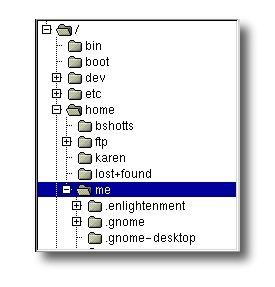
\includegraphics[width=2.5in]{images/1.png}
\caption{File system tree as shown by a graphical file manager}
\label{fig_sim}
\end{figure}

大多数人都可能熟悉图形文件管理器,它描述了文件系统树的结构,正如图1所示。 注意通常,这是一棵倒置的树,也就是说,树根在最上面,而各个枝干在下面展开。

\par 然而,命令行没有图片,所以我们需要考虑用不同的方法,在文件系统树中跳转。

\par 把文件系统想象成一个迷宫形状,就像一棵倒立的大树,我们站在迷宫的中间位置。 在任意时刻,我们处于一个目录里面,我们能看到这个目录包含的所有文件, 以及通往上面目录(父目录)的路径,和下面的各个子目录。我们所在的目录则称为 当前工作目录。我们使用 pwd(打印工作目录)命令,来显示当前工作目录。

\begin{lstlisting}
[me@linuxbox ~]$ pwd
/home/me
\end{lstlisting}

\par 当我们首次登录系统后,(或者启动终端仿真器会话后),当前工作目录设置成主目录。 每个用户都有他自己的主目录,当用户以普通用户的身份操控系统时,主目录是唯一 允许用户编写文件的地方。



\section{列出目录内容} % (fold)
\label{sec:列出目录内容}

列出一个目录包含的文件及子目录,使用 ls 命令。

\begin{lstlisting}
[me@linuxbox ~]$ ls
Desktop Documents Music Pictures Public Templates Videos
\end{lstlisting}

\par 实际上,用 ls 命令可以列出任一个目录的内容,而不只是当前工作目录的内容。 ls 命令还能完成许多有趣的事情。在下一章节,我们将介绍更多关于 ls 的知识。
% section 列出目录内容 (end)

\section{更改当前工作目录} % (fold)
\label{sec:更改当前工作目录}
\par 要更改工作目录(此刻,我们站在树形迷宫里面),我们用 cd 命令。输入 cd, 然后输入你想要的工作目录的路径名,就能实现愿望。路径名就是沿着目录树的分支 到达想要的目录,期间所经过的路线。路径名可通过两种方式来指定,一个是绝对路径, 另一个是相对路径。首先处理绝对路径。

\subsection{绝对路径} % (fold)
\label{ssub:绝对路径}
绝对路径开始于根目录,紧跟着目录树的一个个分支,一直到达期望的目录或文件。 例如,你的系统中有一个目录,大多数系统程序都安装在这个目录下。这个目录的 路径名是 /usr/bin。它意味着从根目录(用开头的“/”表示)开始,有一个叫 “usr” 的 目录包含了目录 “bin”。
\begin{lstlisting}
[me@linuxbox ~]$ cd /usr/bin
[me@linuxbox bin]$ pwd
/usr/bin
[me@linuxbox bin]$ ls
...Listing of many, many files ...
\end{lstlisting}
\par 我们把工作目录转到 /usr/bin 目录下,里面装满了文件。注意 shell 提示符是怎样改变的。 为了方便,通常设置提示符自动显示工作目录名。
% subsection 绝对路径 (end)

\subsection{相对路径} % (fold)
\label{sub:相对路径}
绝对路径从根目录开始,直到它的目的地,而相对路径开始于工作目录。 一对特殊符号来表示相对位置,在文件系统树中。这对特殊符号是 ``.'' (点) 和 ``..'' (点点)。

\par 符号 ``.'' 指的是工作目录,``..'' 指的是工作目录的父目录。下面的例子说明怎样使用它。 再次更改工作目录到 /usr/bin:
\begin{lstlisting}
[me@linuxbox ~]$ cd /usr/bin
[me@linuxbox bin]$ pwd
/usr/bin
\end{lstlisting}

\par 好的,比方说更改工作目录到 /usr/bin 的父目录 /usr。可以通过两种方法来实现。或者使用绝对路径名:

\begin{lstlisting}
[me@linuxbox bin]$ cd /usr
[me@linuxbox usr]$ pwd
/usr
\end{lstlisting}

\par 或者, 使用相对路径:

\begin{lstlisting}
[me@linuxbox bin]$ cd ..
[me@linuxbox usr]$ pwd
/usr
\end{lstlisting}

\par 两种不同的方法,一样的结果。我们应该选哪一个呢? 输入量最少的那个。

\par 同样地,从目录/usr/到/usr/bin 也有两种途径。或者使用绝对路径:

\begin{lstlisting}
[me@linuxbox usr]$ cd /usr/bin
[me@linuxbox bin]$ pwd
/usr/bin
\end{lstlisting}

\par 或者,用相对路径:

\begin{lstlisting}
[me@linuxbox usr]$ cd ./bin
[me@linuxbox bin]$ pwd
/usr/bin
\end{lstlisting}

\par 有一件很重要的事,我必须指出来。在几乎所有的情况下,你可以省略”./”。它是隐含地。输入:
\begin{lstlisting}
[me@linuxbox usr]$ cd bin
\end{lstlisting}

\par 实现相同的效果,如果不指定一个文件的目录,那它的工作目录会被假定为当前工作目录。

% subsection 相对路径 (end)

\subsubsection{有用的快捷键} % (fold)
\label{ssub:有用的快捷键}
在表2-1中,列举出了一些快速改变当前工作目录的有效方法。


\begin{table}[ht!]
% increase table row spacing, adjust to taste
%\renewcommand{\arraystretch}{1.2}
\caption{cd 快捷键}
\label{table_example}
\centering
\begin{tabular}{c|c}
\hline
%\begin{tabular}{|p{0.18\textwidth}|p{0.36\textwidth}|p{0.36\textwidth}|}
 快捷键 & 运行结果 \\
\hline
  cd	& 更改工作目录到主目录。 \\
  cd -	& 更改工作目录到先前的工作目录。\\
cd ~user\_name	& 更改工作目录到用户主目录。例如, cd ~bob 会更改工作目录到用户“bob”的主目录。\\
\hline
\end{tabular}
\end{table}

% subsubsection 有用的快捷键 (end)
\fboxrule=6pt \fboxsep=4pt
\begin{colorboxed}[boxcolor=lightgray,bgcolor=white]
\subsubsection{关于文件名的重要规则}
\begin{enumerate}
	\item 以 ``.'' 字符开头的文件名是隐藏文件。这仅表示,ls 命令不能列出它们, 除非使用 ls -a 命令。当你创建帐号后,几个配置帐号的隐藏文件被放置在 你的主目录下。稍后,我们会仔细研究一些隐藏文件,来定制你的系统环境。 另外,一些应用程序也会把它们的配置文件以隐藏文件的形式放在你的主目录下面。
	\item 文件名和命令名是大小写敏感的。文件名 “File1” 和 “file1” 是指两个不同的文件名。
	\item Linux 没有“文件扩展名”的概念,不像其它一些系统。可以用你喜欢的任何名字 来给文件起名。文件内容或用途由其它方法来决定。虽然类似 Unix 的操作系统, 不用文件扩展名来决定文件的内容或用途,但是应用程序会。
	\item 虽然 Linux 支持长文件名,文件名可能包含空格,标点符号,但标点符号仅限 使用 ``.'',``-'',下划线。最重要的是,不要在文件名中使用空格。如果你想表示词与 词间的空格,用下划线字符来代替。过些时候,你会感激自己这样做。
\end{enumerate}
\end{colorboxed}
% section 更改当前工作目录 (end)




%第三章
%% Public domain image from
%% http://www.public-domain-image.com/still-life/slides/cherry-tomatos.html
\renewcommand\chapterillustration{cherry-tomatos}
\chapter{探究操作系统}

既然我们已经知道了如何在文件系统中跳转,是时候开始 Linux 操作系统之旅了。在开始之前,我们先学习一些对研究 Linux 系统有帮助的命令。

\begin{itemize}
	\item ls — 列出目录内容
	\item file — 确定文件类型
	\item less — 浏览文件内容
\end{itemize}

\section{ls 乐趣}

有充分的理由证明,ls 可能是用户最常使用的命令。通过它,我们可以知道目录的内容,以及各种各样重要文件和目录的 属性。正如我们所知道的,只简单的输入 ls 就能看到在当前目录下所包含的文件和子目录列表。

\begin{lstlisting}
[me@linuxbox ~]$ ls
Desktop Documents Music Pictures Publica Templates Videos 
\end{lstlisting}

\par 除了当前工作目录以外,也可以列出指定目录的内容,就像这样:

\begin{lstlisting}
me@linuxbox ~]$ ls /usr
bin games   kerberos    libexec  sbin   src
etc include lib         local    share  tmp 
\end{lstlisting}

\par 甚至可以列出多个指定目录的内容。在这个例子中,将会列出用户主目录(用字符“~”代表)和/usr 目录的内容:

\begin{lstlisting}
[me@linuxbox ~]$ ls ~ /usr
/home/me:
Desktop  Documents  Music  Pictures  Public  Templates  Videos

/usr:
bin  games      kerberos  libexec  sbin   src
etc  include    lib       local    share  tmp 
\end{lstlisting}

\par 我们也可以改变输出格式,来得到更多的细节:

\begin{lstlisting}
[me@linuxbox ~]$ ls -l
total 56
drwxrwxr-x 2  me  me  4096  2007-10-26  17:20  Desktop
drwxrwxr-x 2  me  me  4096  2007-10-26  17:20  Documents
drwxrwxr-x 2  me  me  4096  2007-10-26  17:20  Music
drwxrwxr-x 2  me  me  4096  2007-10-26  17:20  Pictures
drwxrwxr-x 2  me  me  4096  2007-10-26  17:20  Public
drwxrwxr-x 2  me  me  4096  2007-10-26  17:20  Templates
drwxrwxr-x 2  me  me  4096  2007-10-26  17:20  Videos
\end{lstlisting}

\par 使用 ls 命令的“-l”选项,则结果以长模式输出。


\subsection{选项和参数}
我们将学习一个非常重要的知识点,大多数命令是如何工作的。命令名经常会带有一个或多个用来更正命令行为的选项, 更进一步,选项后面会带有一个或多个参数,这些参数是命令作用的对象。所以大多数命令看起来像这样:

\begin{lstlisting}
command -options arguments
\end{lstlisting}

\par 大多数命令使用的选项,是由一个中划线加上一个字符组成,例如,“-l”,但是许多命令,包括来自于 GNU 项目的命令,也支持长选项,长选项由两个中划线加上一个字组成。当然, 许多命令也允许把多个短选项串在一起使用。下面这个例子,ls 命令有两个选项, “l” 选项产生长格式输出,“t”选项按文件修改时间的先后来排序。

\begin{lstlisting}
[me@linuxbox ~]$ ls -lt
\end{lstlisting}

\par 加上长选项 “–reverse”,则结果会以相反的顺序输出:

\begin{lstlisting}
[me@linuxbox ~]$ ls -lt --reverse
\end{lstlisting}

\par ls 命令有大量的选项。表3-1列出了最常使用的选项。

\begin{table}[ht!]
% increase table row spacing, adjust to taste
%\renewcommand{\arraystretch}{1.2}
\caption{ls 命令选项}
\label{table_example}
\centering
\begin{tabular}{p{1.5cm}p{3.5cm}p{10cm}}
%\begin{tabular}{c|c|c}
\hline
%\begin{tabular}{|p{0.18\textwidth}|p{0.36\textwidth}|p{0.36\textwidth}|}
 选项 & 长选项 & 描述 \\
\hline
 -a & --all & 列出所有文件,甚至包括文件名以圆点开头的隐藏文件。 \\
-d & --directory & 通常,如果指定了目录名,ls 命令会列出这个目录中的内容,而不是目录本身。 把这个选项与-l 选项结合使用,可以看到所指定目录的详细信息,而不是目录中的内容。\\
-F & --classify	& 这个选项会在每个所列出的名字后面加上一个指示符。例如,如果名字是 目录名,则会加上一个``/''字符。 \\
-h & --human-readable & 以长格式列出。以人们可读的格式,而不是以字节数来显示文件的大小。\\
-l & & 以长格式显示结果。\\
-r & --reverse & 以相反的顺序来显示结果。通常,ls 命令的输出结果按照字母升序排列。 \\
-S & & 命令输出结果按照文件大小来排序。\\
-t & & 按照修改时间来排序。\\
\hline
\end{tabular}
\end{table}


\subsection{深入研究长格式输出}
正如我们先前知道的,“-l”选项导致 ls 的输出结果以长格式输出。这种格式包含大量的有用信息。下面的例子目录来自 于 Ubuntu 系统:
(注:由于排版原因,删除了原文的的一部分.)
\begin{lstlisting}
-rw-r--r-- 1 root root 3576296 2007-04-03 11:05 Experience ubuntu.ogg
-rw-r--r-- 1 root root 1186219 2007-04-03 11:05 kubuntu-leaflet.png 
-rw-r--r-- 1 root root   47584 2007-04-03 11:05 logo-Edubuntu.png 
-rw-r--r-- 1 root root   44355 2007-04-03 11:05 logo-Kubuntu.png
-rw-r--r-- 1 root root   34391 2007-04-03 11:05 logo-Ubuntu.png
-rw-r--r-- 1 root root   32059 2007-04-03 11:05 oo-cd-cover.odf
\end{lstlisting}

\par 选一个文件,来看一下各个输出字段的含义(表3-2):

\begin{table}[ht!]
% increase table row spacing, adjust to taste
%\renewcommand{\arraystretch}{1.2}
\caption{ls 长格式列表的字段}
\label{table_example}
\centering
\begin{tabular}{p{4cm}p{11cm}}
%\begin{tabular}{c|c|c}
\hline
%\begin{tabular}{|p{0.18\textwidth}|p{0.36\textwidth}|p{0.36\textwidth}|}
 字段 & 含义 \\
 \hline 
 -rw-r--r--	& 对于文件的访问权限。第一个字符指明文件类型。在不同类型之间,开头的“-”说明是一个普通文件,“d”表明是一个目录。其后三个字符是文件所有者的访问权限,再其后的三个字符是文件所属组中成员的访问权限,最后三个字符是其他所 有人的访问权限。这个字段的完整含义将在第十章讨论。\\
1 & 文件的硬链接数目。参考随后讨论的关于链接的内容。 \\
root & 文件属主的用户名。 \\
root & 文件所属用户组的名字。 \\
32059 & 以字节数表示的文件大小。\\
2007-04-03 11:05 & 上次修改文件的时间和日期。 \\
oo-cd-cover.odf	& 文件名。 \\
\hline

\end{tabular}
\end{table}

\section{确定文件类型} % (fold)
\label{sec:确定文件类型}
随着探究操作系统的进行,知道文件包含的内容是很有用的。我们将用 file 命令来确定文件的类型。我们之前讨论过, 在 Linux 统中,并不要求文件名来反映文件的内容。然而,一个类似 “picture.jpg” 的文件名,我们会期望它包含 JPEG 压缩图像,但 Linux 却不这样要求它。可以这样调用 file 命令:

\begin{lstlisting}
file filename
\end{lstlisting}

\par 当调用 file 命令后,file 命令会打印出文件内容的简单描述。例如:

\begin{lstlisting}
[me@linuxbox ~]$ file picture.jpg
picture.jpg: JPEG image data, JFIF standard 1.01
\end{lstlisting}

\par 有许多类型的文件。事实上,在类似于 Unix 操作系统中比如说 Linux,有个普遍的观念就是“任何东西都是一个文件”。 随着课程的进行,我们将会明白这句话的真谛。

\par 虽然系统中许多文件格式是熟悉的,例如 MP3和 JPEG 文件,但也有一些文件格式比较含蓄,极少数文件相当陌生。


% section 确定文件类型 (end)

\section{用 less 浏览文件内容} % (fold)
\label{sec:用_less_浏览文件内容}

less 命令是一个用来浏览文本文件的程序。纵观 Linux 系统,有许多人类可读的文本文件。less 程序为我们检查文本文件 提供了方便。

\fboxrule=6pt \fboxsep=4pt
\begin{colorboxed}[boxcolor=lightgray,bgcolor=white]
\subsection{什么是``文本''}
在计算机中,有许多方法可以表达信息。所有的方法都涉及到,在信息与一些数字之间确立一种关系,而这些数字可以 用来表达信息。毕竟,计算机只能理解数字,这样所有的数据都被转换成数值表示法。

\par 有些数值表达法非常复杂(例如压缩的视频文件),而其它的就相当简单。最早也是最简单的一种表达法,叫做 ASCII 文本。ASCII(发音是"As-Key")是美国信息交换标准码的简称。这是一个简单的编码方法,它首先 被用在电传打字机上,用来实现键盘字符到数字的映射。

\par 文本是简单的字符与数字之间的一对一映射。它非常紧凑。五十个字符的文本翻译成五十个字节的数据。文本只是包含 简单的字符到数字的映射,理解这点很重要。它和一些文字处理器文档不一样,比如说由微软和 OpenOffice.org 文档 编辑器创建的文件。这些文件,和简单的 ASCII 文件形成鲜明对比,它们包含许多非文本元素,来描述它的结构和格式。 普通的 ASCII 文件,只包含字符本身,和一些基本的控制符,像制表符,回车符及换行符。纵观 Linux 系统,许多文件 以文本格式存储,也有许多 Linux 工具来处理文本文件。甚至 Windows 也承认这种文件格式的重要性。著名的 NOTEPAD.EXE 程序就是一个 ASCII 文本文件编辑器。
\end{colorboxed}

\par 为什么我们要查看文本文件呢? 因为许多包含系统设置的文件(叫做配置文件),是以文本格式存储的,阅读它们 可以更深入的了解系统是如何工作的。另外,许多系统所用到的实际程序(叫做脚本)也是以这种格式存储的。 在随后的章节里,我们将要学习怎样编辑文本文件,为的是修改系统设置,还要学习编写自己的脚本文件,但现在我们只是看看它们的内容而已。

\par less 命令是这样使用的:

\begin{lstlisting}
less filename
\end{lstlisting}

\par 一旦运行起来,less 程序允许你前后滚动文件。例如,要查看一个定义了系统中全部用户身份的文件,输入以下命令:
\begin{lstlisting}
[me@linuxbox ~]$ less /etc/passwd
\end{lstlisting}

\par 一旦 less 程序运行起来,我们就能浏览文件内容了。如果文件内容多于一页,那么我们可以上下滚动文件。按下“q”键, 退出 less 程序。

\par 下表列出了 less 程序最常使用的键盘命令。
\begin{table}[ht!]
% increase table row spacing, adjust to taste
%\renewcommand{\arraystretch}{1.2}
\caption{less 命令}
\label{table3}
\centering
\begin{tabular}{p{4cm}p{11cm}}
%\begin{tabular}{c|c|c}
\hline
%\begin{tabular}{|p{0.18\textwidth}|p{0.36\textwidth}|p{0.36\textwidth}|}
命令 & 行为\\

\hline
Page UP or b &	向后翻滚一页\\
Page Down or space & 向前翻动一页 \\
UP Arrow & 向前移动一行\\
Down Arrow &	向后移动一行\\
G	& 移动到最后一行\\
1G or g	& 移动到开头一行\\
/charaters	& 向前查找指定的字符串\\
n	& 向前查找下一个出现的字符串,这个字符串是之前所指定查找的\\
h	& 显示帮助屏幕\\
q	& 退出 less 程序\\
\hline
\end{tabular}
\end{table}

\fboxrule=6pt \fboxsep=4pt
\begin{colorboxed}[boxcolor=lightgray,bgcolor=white]
\subsection{less 就是 more(禅语:色即是空)}

ess 程序是早期 Unix 程序 more 的改进版。“less” 这个名字,对习语 “less is more” 开了个玩笑, 这个习语是现代主义建筑师和设计者的座右铭。

\par less 属于”页面调度器”程序类,这些程序允许通过页方式,在一页中轻松地浏览长长的文本文档。然而 more 程序只能向前分页浏览,而 less 程序允许前后分页浏览,它还有很多其它的特性。
\end{colorboxed}


% section 用_less_浏览文件内容 (end)


\section{旅行指南} % (fold)
\label{sec:旅行指南}

Linux 系统中,文件系统布局与类似 Unix 系统的文件布局很相似。实际上,一个已经发布的标准, 叫做 Linux 文件系统层次标准,详细说明了这种设计模式。不是所有Linux发行版都根据这个标准,但 大多数都是。

\par 下一步,我们将在文件系统中游玩,来了解 Linux 系统的工作原理。这会给你一个温习跳转命令的机会。 我们会发现很多有趣的文件都是普通的可读文本。将开始旅行,做做以下练习:
\begin{enumerate}
	\item cd 到给定目录
	\item 列出目录内容 ls -l
	\item 如果看到一个有趣的文件,用 file 命令确定文件内容
	\item 如果文件看起来像文本,试着用 less 命令浏览它
\end{enumerate}
\fboxrule=3pt \fboxsep=2pt
\begin{colorboxed}[boxcolor=lightgray,bgcolor=white]
\textbf{记得复制和粘贴技巧!}如果你正在使用鼠标,双击文件名,来复制它,然后按下鼠标中键,粘贴文件名到命令行中。
\end{colorboxed}

\par 在系统中游玩时,不要害怕粘花惹草。普通用户是很难把东西弄乱的。那是系统管理员的工作! 如果一个命令抱怨一些事情,不要管它,尽管去玩别的东西。花一些时间四处走走。 系统是我们自己的,尽情地探究吧。记住在 Linux 中,没有秘密存在! 表3-4仅仅列出了一些我们可以浏览的目录。闲暇时试试看!


% section 旅行指南 (end)



% \section{拓展阅读} % (fold)
\label{sec:拓展阅读2}

\begin{itemize}
	\item 想了解更多关于 Steve Bourne 的故事,Bourne Shell 之父,读一下这篇文章:\\
	\url{http://en.wikipedia.org/wiki/Steve_Bourne}\\
	\item 这是一篇关于在计算机领域里,shells 概念的文章:\\
	\url{http://en.wikipedia.org/wiki/Shell_(computing)}\\
\end{itemize}
% section 拓展阅读 (end)





%背面
%\cleartoverso

%%%%%%%%%%%%%%%%%%%%%%
%% Back cover
%%%%%%%%%%%%%%%%%%%%%%

%% Temporarily enlarge this page to push
%% down the bottom margin
\enlargethispage{3\baselineskip}
\thispagestyle{empty}
%\pagecolor[HTML]{0C0303}
\pagecolor[HTML]{0E0407}

\begin{center}
\begin{minipage}{.8\textwidth}
\color{Cornsilk}\Large\bfseries
\lipsum[1]

\begin{center}
\huge\bfseries\sffamily\color{lime}`So Calming.'
\end{center}

\lipsum[2]

\end{minipage}
\end{center}

\vspace*{\stretch{1}}

\begin{center}
\colorbox{white}{\EANisbn[SC4]}

\vspace*{\baselineskip}

\textbf{\textcolor{LightGoldenrod!50!Gold}{Malaysian \LaTeX\ User Group \textbullet\ \texttt{http://latex-my.blogspot.com}}}

\vspace*{\baselineskip}

\textbf{\textcolor{LightGoldenrod}{Cover Illustration by Dusan Bicanski \textbullet\ \texttt{http://www.public-domain-image.com}}}
\end{center}

\end{document}